\documentclass{article}
\author{Alex Hiller (11850637)}
\title{Linear Algebra, Assignment 4}
\setlength{\parindent}{0cm}
\setlength{\parskip}{0.125cm}
\pagenumbering{gobble}
\usepackage[margin=2.5cm]{geometry} % Formatting
\usepackage{amsmath}                % Mathematics
\usepackage{amssymb}                % Mathematics
\usepackage{esint}                  % Mathematics
\usepackage{listings}               % Listings
\usepackage{color}                  % Listings
\usepackage{courier}                % Listings
\usepackage{circuitikz}             % Circuits
\usepackage{titlesec}               % Section Formatting
\usepackage{graphicx}               % Graphics
\usepackage{stmaryrd}               % \mapsfrom arrow. ↤
\input{/home/polluticorn/GitHub/texTemplates/texMacros}
% Section formatting
\titleformat{\section}{\huge \bfseries}{}{0em}{}[]
\titleformat{\subsection}{\Large \bfseries}{}{0em}{}
\titleformat{\subsubsection}{\bfseries}{}{0em}{}

%%%%%%%%%%%%%%%%%%%%%%%%%%%%%%%%%%%%%%%%%%%%%%%%%%%%%%%%%%%%%%%%%%%%%%%%%%%%%%%%
\begin{document}
\maketitle
\clearpage

%%%%%%%%%%%%%%%%%%%%%%%%%%%%%%%%%%%%%%%%
\section{Question 1}
\[
    \mathbf{a_1} = 
    \begin{bmatrix}
        0 \\ 
        3 \\ 
        4 \\
    \end{bmatrix}
    \quad 
    \mathbf{a_2} =
    \begin{bmatrix}
        1\\
        2\\
        1\\
    \end{bmatrix}
    \quad
    \mathbf{b_1} = 
    \begin{bmatrix}
        1 \\
        2 \\
    \end{bmatrix}
    \quad 
    \mathbf{b_2} = 
    \begin{bmatrix}
        2 \\
        0 \\
    \end{bmatrix}
    \quad 
    \mathbf{b_3} = 
    \begin{bmatrix}
        -1 \\
        1 \\
    \end{bmatrix}
\]


Calculations:


\[
    \mathbf{a_1} -
    4 \mathbf{a_2} =
    \begin{bmatrix}
        0 \\ 3 \\ 4 \\
    \end{bmatrix}
    -4
    \begin{bmatrix}
        1\\ 2\\ 1\\
    \end{bmatrix}
    =
    \begin{bmatrix}
        0 \\ 3 \\ 4 \\
    \end{bmatrix}
    -
    \begin{bmatrix}
        4\\ 8\\ 4\\
    \end{bmatrix}
    =
    \begin{bmatrix}
        -4 \\ -5 \\ 0 \\
    \end{bmatrix}
\]


\[
    \mathbf{b_1} 
    +
    2 \mathbf{b_3} 
    =     
    \begin{bmatrix}
        1 \\ 2 \\
    \end{bmatrix}
    +
    2
    \begin{bmatrix}
        -1 \\ 1 \\
    \end{bmatrix}
    =
    \begin{bmatrix}
        1 \\ 2 \\
    \end{bmatrix}
    +
    \begin{bmatrix}
        -2 \\ 2 \\
    \end{bmatrix}
    =
    \begin{bmatrix}
        -1 \\ 4 \\
    \end{bmatrix}
\]


\[
(\mathbf{a_2} +
3 \mathbf{b_2}  )
\ \text{is undefined}
\]


\[
    \mathbf{b_1} +
    \mathbf{b_2} -
    3
    \mathbf{b_3} 
    \ = \
    \begin{bmatrix}
        1 \\ 2 \\
    \end{bmatrix}
    +
    \begin{bmatrix}
        2 \\ 0 \\
    \end{bmatrix}
    -
    3
    \begin{bmatrix}
        -1 \\ 1 \\
    \end{bmatrix}
    \ = \
    \begin{bmatrix}
        3 \\ 2 \\
    \end{bmatrix}
    -
    \begin{bmatrix}
        -3 \\ 3 \\
    \end{bmatrix}
    \ = \
    \begin{bmatrix}
        6 \\ -1 \\
    \end{bmatrix}
\]

%%%%%%%%%%%%%%%%%%%%%%%%%%%%%%%%%%%%%%%%


%%%%%%%%%%%%%%%%%%%%%%%%%%%%%%%%%%%%%%%%
\clearpage
\section{Question 2}
$$
\begin{bmatrix}
    2 & -2 \\
    3 & 3\\
    4 & -4\\
\end{bmatrix}
\begin{bmatrix}
    x_1 \\
    x_2\\
\end{bmatrix}
=
\begin{bmatrix}
    b_1 \\
    b_2 \\
    b_3 \\
\end{bmatrix}
$$

Set up an augmented matrix:
\[
    \begin{bmatrix}
        2 & -2 & b_1 \\
        3 &  3 & b_2 \\
        4 & -4 & b_3 \\
    \end{bmatrix}
\]

Reduce to row echelon form:

\[
    R_3 \mapsfrom (R_3 - 2 R_1)
    \Rightarrow
    \begin{bmatrix}
        2 & -2 & b_1       \\
        3 &  3 & b_2       \\
        0 &  0 & b_3-2 b_1 \\
    \end{bmatrix}
.\]


\[
    R_2 \mapsfrom (R_2 - \frac{3}{2} R_1)
    \Rightarrow
    \begin{bmatrix}
        2 & -2 & b_1                    \\
        0 &  6 & b_2 - \frac{3}{2} b_1  \\
        0 &  0 & b_3-2 b_1              \\
    \end{bmatrix}
.\]

This means that to have a consistent $\mathbf{b}$, we must have: $b_3 - 2 b_1 = 0$

Leading us to: 
\[
    \begin{bmatrix}
        b_1 \\
        b_2 \\
        b_3 \\
    \end{bmatrix}
    = 
    \begin{bmatrix}
        b_1 \\
        b_2 \\
        2 b_1 \\
    \end{bmatrix}
    = 
    b_1
    \begin{bmatrix}
        1 \\ 0 \\ 2 \\
    \end{bmatrix}
    +
    b_2
    \begin{bmatrix}
        0 \\ 1 \\ 0 \\
    \end{bmatrix}
    =
    b_1
    \mathbf{u}
    +
    b_2
    \mathbf{v}
.\]

Meaning that a set of solutions that are consistent with the system would lie in
a plane made of linear combinations of $\mathbf{u}$ and $\mathbf{v}$.

Visual, geometric interpretation of linear combinations of $\mathbf{u}$ and $\mathbf{v}$:

\begin{figure}[!htbp]
    \centering
    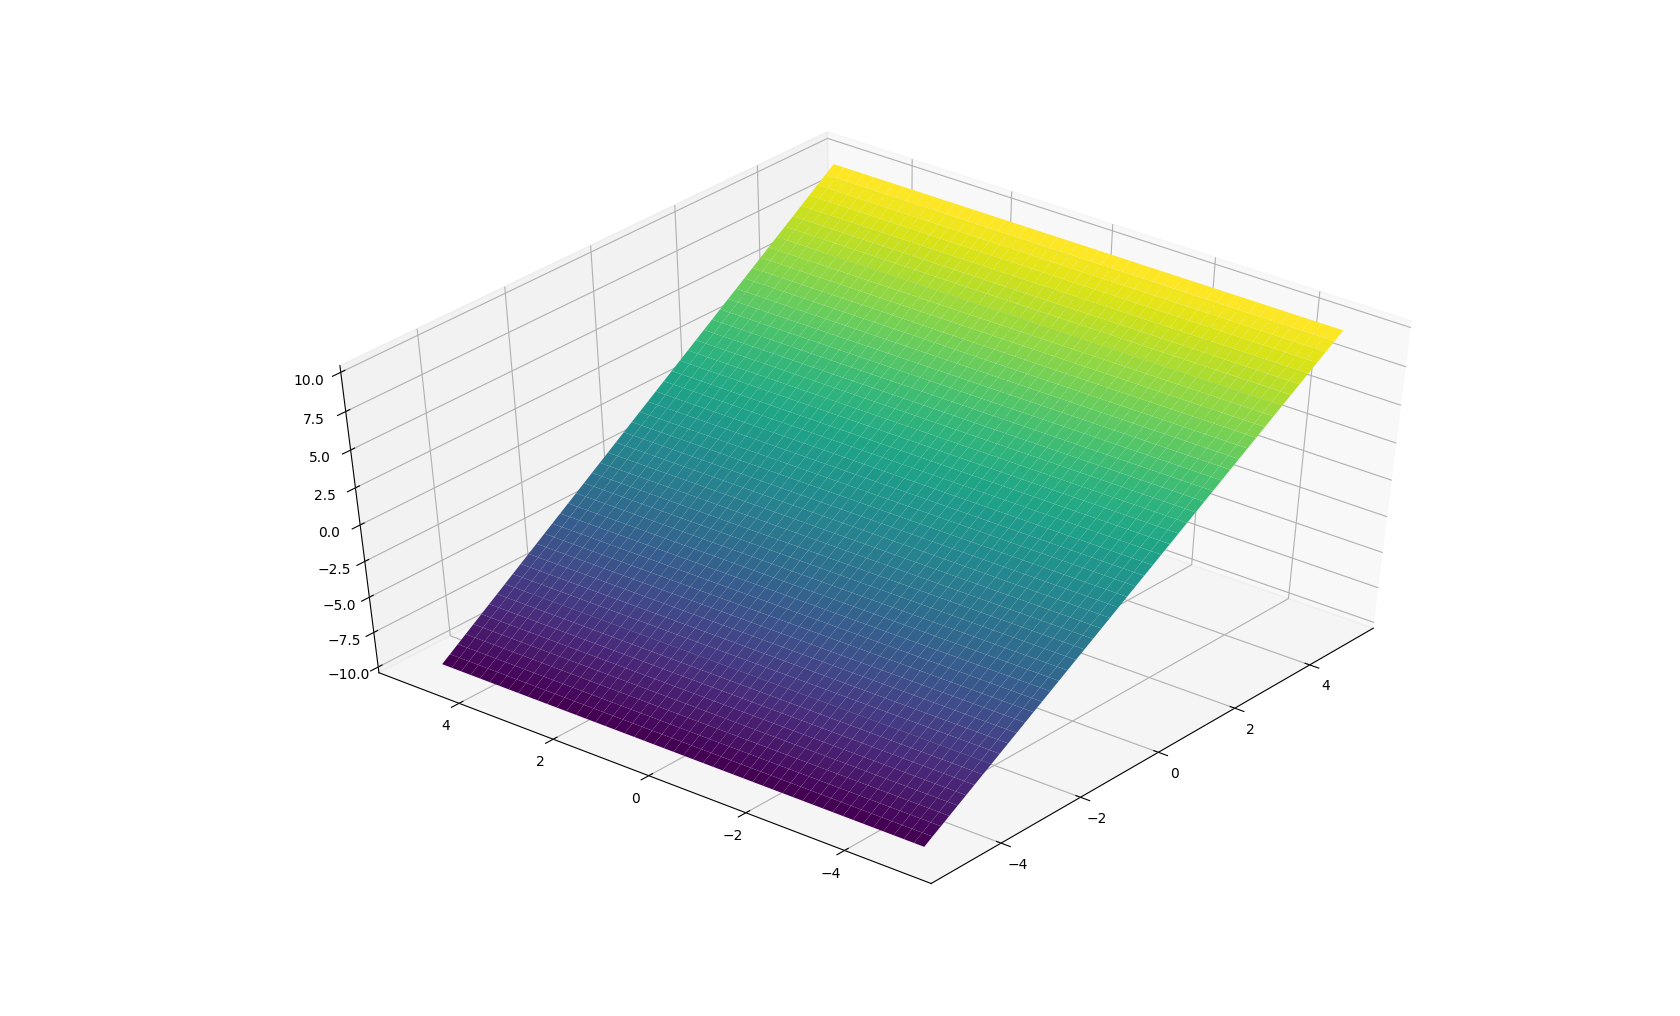
\includegraphics[width=0.8\textwidth]{plane.png}
\end{figure}

%%%%%%%%%%%%%%%%%%%%%%%%%%%%%%%%%%%%%%%%


%%%%%%%%%%%%%%%%%%%%%%%%%%%%%%%%%%%%%%%%
\clearpage
\section{Question 3}
\[
\mathbf{v_1} =
\begin{bmatrix}
    3 \\
    2 \\
    2 \\
\end{bmatrix}
\quad
\mathbf{v_2} = 
\begin{bmatrix}
    2 \\
    -1 \\
    -1 \\
\end{bmatrix}
\quad
\mathbf{v_3} = 
\begin{bmatrix}
    3 \\
    3 \\
    3 \\
\end{bmatrix}
\quad
\mathbf{v_4} = 
\begin{bmatrix}
    2 \\
    0 \\
    1 \\
\end{bmatrix}
.\]

First, we form an augmented matrix of the vectors:

\[
    \mathbf{A} 
    =
    \begin{bmatrix} \
        \mathbf{v_1} \
        \mathbf{v_2} \
        \mathbf{v_3} \
        \mathbf{v_4} \
    \end{bmatrix}
    = 
    \begin{bmatrix}
        3 &  2 & 3 & 2 \\
        2 & -1 & 3 & 0 \\
        2 & -1 & 3 & 1 \\
    \end{bmatrix}
.\]

Getting into Reduced-Row-Echelon Form:

\[
    \text{rref}(\mathbf{A})
    =
    \begin{bmatrix}
        1 &  0 & \frac{9}{7}  & 0 \\
        0 &  1 & \frac{-3}{7} & 0 \\
        0 &  0 & 0            & 1 \\
    \end{bmatrix}
.\]


Before continuing with our investigation we must define the term 'rank'. 

The '\textit{rank}' of a matrix is defined as: \textit{The dimension of vector space spanned
by its columns.}

We can see that the matrix has three pivots, (which, as a side-note, also means that it is of full-rank).

Hence if the matrix is of rank 3, then this means that the matrix spans
3-dimensional vector space, $\mathbb{R}^{3}$.

Therefore: 

\[
    \text{Span} \{
    \mathbf{v_1},\
    \mathbf{v_2},\
    \mathbf{v_3},\
    \mathbf{v_4} \} 
    \in 
    \mathbb{R}^{3}
.\]

%%%%%%%%%%%%%%%%%%%%%%%%%%%%%%%%%%%%%%%%

%%%%%%%%%%%%%%%%%%%%%%%%%%%%%%%%%%%%%%%%
\clearpage
\section{Question 4}
\[
\begin{bmatrix}
    1 & 1 & 4 & 1 \\
    1 & 2 & 9 & 0 \\
    2 & 1 & 3 & 3 \\
\end{bmatrix}
\begin{bmatrix}
    x_1 \\ x_2 \\ x_3 \\ x_4 \\
\end{bmatrix}
=
\begin{bmatrix}
    0 \\ 0 \\ 0 \\
\end{bmatrix}
.\]


Forming an augmented matrix:


\[
    \mathbf{A} 
    = 
    \begin{bmatrix}
        1 & 1 & 4 & 1 & 0 \\
        1 & 2 & 9 & 0 & 0 \\
        2 & 1 & 3 & 3 & 0 \\
    \end{bmatrix}
.\]


Getting $\mathbf{A}$ into Reduced-Row-Echelon-Form:


\[
    \text{rref}(\mathbf{A})
    = 
    \begin{bmatrix}
        1 & 0 &-1 & 2 & 0 \\
        0 & 1 & 5 &-1 & 0 \\
        0 & 0 & 0 & 0 & 0 \\
    \end{bmatrix}
.\]


\[
    \text{Basic variables} = \{ x_1, x_2 \}
.\]


\[
    \text{Free variables} = \{ x_3, x_4 \}
.\]


So, to satisfy our system, we must have a certain set of values for $\mathbf{x}$
that satisfy the system and equal $\mathbf{0}$.

That set of x-values is given by our row-reduction.

Expressing the basic variables in terms of the free variables

\[
    \begin{bmatrix}
        x_1 \\ x_2 \\ x_3 \\ x_4 \\
    \end{bmatrix}
    =
    \begin{bmatrix}
        x_3 - 2 x_4     \\
        -5 x_3 + x_4    \\ 
        x_3 \\ x_4      \\
    \end{bmatrix}
    = \
    x_3
    \begin{bmatrix}
        1 \\ -5 \\ 1 \\ 0 \\
    \end{bmatrix}
    + 
    x_4
    \begin{bmatrix}
        -2 \\ 1 \\ 0 \\ 1 \\
    \end{bmatrix}
    +
    \begin{bmatrix}
        0 \\ 0 \\ 0 \\ 0 \\
    \end{bmatrix}
.\]


Hence the solution set is:

\[
    \text{Span} \
    \bigg\{ 
    \begin{bmatrix}
        1 \\ -5 \\ 1 \\ 0 \\
    \end{bmatrix}
    ,
    \begin{bmatrix}
        -2 \\ 1 \\ 0 \\ 1 \\
    \end{bmatrix}
    \bigg\}
.\]
%%%%%%%%%%%%%%%%%%%%%%%%%%%%%%%%%%%%%%%%

%%%%%%%%%%%%%%%%%%%%%%%%%%%%%%%%%%%%%%%%
\clearpage
\section{Question 5}
\[
\begin{bmatrix}
    1 & 1 & -1 & -2 \\
    2 & -1 & -3  & -5 \\
    1 & 2 & -6 & -7  \\
\end{bmatrix}
\begin{bmatrix}
    x_1 \\ x_2 \\ x_3 \\ x_4 \\
\end{bmatrix}
=
\begin{bmatrix}
    1 \\ 7 \\ -6 \\
\end{bmatrix}
.\]

Forming an augmented matrix:
\[
    \mathbf{A}
    =
    \begin{bmatrix}
        1 & 1 & -1  & -2 & 1  \\
        2 & -1 & -3 & -5 & 7  \\
        1 & 2 & -6  & -7 & -6 \\
    \end{bmatrix}
.\]

Transforming to Reduced-Row-Echelon form:
\[
    \text{rref}(\mathbf{A})
    =
    \begin{bmatrix}
        1 & 0 & 0 & -1  & 4  \\
        0 & 1 & 0 &  0  & -2 \\
        0 & 0 & 1 &  1  & 1  \\
    \end{bmatrix}
.\]
 
Therefore:

\[
    \text{Basic variables} = \{ x_1, x_2, x_3 \}
.\]


\[
    \text{Free variable} = \{ x_4 \}
.\]


\[
    \begin{bmatrix}
        x1 \\ x2 \\ x3 \\ x4 \\
    \end{bmatrix}
    = 
    \begin{bmatrix}
        x_4 + 4     \\
        -2          \\
        - x_4 + 1   \\
        x_4         \\
    \end{bmatrix}
    = 
    x_4
    \begin{bmatrix}
        1 \\ 0 \\ -1 \\ 1 \\ 
    \end{bmatrix}
    + 
    \begin{bmatrix}
        4 \\ -2 \\ 1 \\ 0 \\
    \end{bmatrix}
.\]

Hence the solutions lie on a line (?) in 4D space.






%%%%%%%%%%%%%%%%%%%%%%%%%%%%%%%%%%%%%%%%


\end{document}































